\chapter{Implementação}

\section{Método de implementação}
Conforme citado, foi utilizada a \textbf{Infraestrutura como Código (IaC)} para a construção da nossa arquitetura. O código será detalhado para facilitar o entendimento e servir como documentação para futuras manutenções ou novas implementações. A estrutura geral de cada recurso, incluindo seu nome, tipo e o bloco de propriedades, segue um padrão global no CloudFormation. Por isso, a partir de agora, focaremos apenas nas propriedades que são cruciais e específicas para cada recurso, evitando repetições e tornando a leitura mais objetiva.

\Needspace{2\baselineskip}
\section{VPC}
Com esse trecho, fizemos a criação do nosso recurso Virtual Private Cloud (VPC).
\begin{lstlisting}[language=yaml, float=htbp,]
 VPC:
   Type: AWS::EC2::VPC
   Properties:
     CidrBlock: 10.16.0.0/16
     EnableDnsSupport: true
     EnableDnsHostnames: true
     Tags: [{ Key: Name, Value: TCC-VPC }]
\end{lstlisting}

A seguir, detalhamos cada uma das propriedades do código da VPC:
\begin{description}
    \item[\textbf{VPC:}] É o nome que demos ao recurso. Ele serve como um identificador único, permitindo que outros recursos (como as subnets) o referenciem futuramente no mesmo código.
    \item[\textbf{Type: AWS::EC2::VPC}] Esta é a declaração formal do recurso, especificando que estamos criando uma \textbf{Virtual Private Cloud}.
    \item[\textbf{Properties:}] Este bloco contém todas as configurações e propriedades específicas para o recurso VPC.
    \item[\textbf{CidrBlock:}] Define o bloco de endereços IP da nossa rede e o seu respectivo \textit{range}.
    \item[\textbf{EnableDnsSupport e EnableDnsHostnames:}] Ambas as propriedades, quando definidas como \texttt{true}, ativam o suporte a DNS, permitindo que os recursos dentro da VPC se comuniquem usando nomes de domínio em vez de apenas endereços IP.
    \item[\textbf{Tags:}] São etiquetas ou rótulos que auxiliam na identificação e organização do recurso no console da AWS, de forma visual e intuitiva.
\end{description}
\section{Subnets}
Após a criação da nossa rede principal (\textbf{VPC}), o próximo passo é dividi-la em sub-redes ou \textbf{subnets}. Para o nosso projeto, criamos uma subnet pública (para recursos com acesso à internet) e uma privada (para recursos que devem permanecer isolados).

Para garantir alta disponibilidade e organização, nossa infraestrutura de rede foi planejada com seis subnets distribuídas em duas Zonas de Disponibilidade (AZs). Essa estrutura proporciona redundância e resiliência a falhas.

\begin{enumerate}
    \item Subnet Pública na primeira AZ, para recursos com acesso direto à internet.
    \item Subnet Pública na segunda AZ, servindo ao mesmo propósito na AZ secundária.
    \item Subnet Privada para os containers na primeira AZ, isolando a aplicação da internet.
    \item Subnet Privada para os containers na segunda AZ, garantindo a resiliência do ambiente.
    \item Subnet Privada para o banco de dados na primeira AZ, assegurando o máximo de isolamento e segurança.
    \item Subnet Privada para o banco de dados na segunda AZ, com a mesma finalidade na AZ de backup.
\end{enumerate}

\subsection{Subnet Pública}
Esta subnet foi criada para hospedar recursos que precisam ser acessíveis publicamente, como servidores web ou balanceadores de carga.

\Needspace{2\baselineskip}
\begin{lstlisting}[language=yaml, float=htbp]
 PublicSubnetA:
   Type: AWS::EC2::Subnet
   Properties:
     AvailabilityZone: !Select [0, !GetAZs '']
     VpcId: !Ref VPC
     CidrBlock: 10.16.0.0/20
     Tags: [{ Key: Name, Value: PublicSubnetA }]
\end{lstlisting}


\begin{description}
\item[\textbf{VpcId: !Ref VPC}] Esta propriedade é crucial. Ela utiliza a função intrínseca \texttt{!Ref} para referenciar o recurso \textbf{VPC} que definimos anteriormente. Isso garante que esta subnet seja criada dentro do ambiente de rede que configuramos.
\item[\textbf{AvailabilityZone: !Select [0, !GetAZs ' ']}] O campo \texttt{AvailabilityZone} define em qual Zona de Disponibilidade a Subnet será criada. Usamos a função \texttt{!Select [0, !GetAZs ' ']} para selecionar a primeira Zona de Disponibilidade disponível na região, considerando que a contagem de índices começa em 0.
\item[\textbf{CidrBlock:}] Define o bloco de endereços IP para esta subnet. É importante notar que este bloco de endereços, \texttt{10.16.0.0/20}, é um sub-bloco extraído do \textit{range} maior da nossa VPC, \texttt{10.16.0.0/16}, garantindo que ele não se sobreponha a outras subnets.
\end{description}

\subsection{Vínculo do IGW com a VPC}
Percebemos que a exposição da subnet não é decidida no momento de sua criação, somente quando a associamos a recursos que se conectam com a internet pública, como o IGW, como mostrado a seguir.

\Needspace{2\baselineskip}
\begin{lstlisting}[language=yaml, float=htbp]
 IGW:
   Type: AWS::EC2::InternetGateway
   Properties:
     Tags: [{ Key: Name, Value: TCC-IGW }]
\end{lstlisting}

\Needspace{2\baselineskip}
\begin{lstlisting}[language=yaml, float=htbp]
 AttachIGW:
   Type: AWS::EC2::VPCGatewayAttachment
   Properties:
     VpcId: !Ref VPC
     InternetGatewayId: !Ref IGW
\end{lstlisting}
Com essa sequência de imagens, podemos observar a criação e o vínculo do nosso Internet Gateway com a nossa VPC, processo que se dá por meio das seguintes características:
\begin{description}
\item [\textbf{VpcId: !Ref VPC}] onde referenciamos a VPC que será vinculada.
\item [\textbf{InternetGatewayId: !Ref IGW}] onde referenciamos o Internet Gateway que será utilizado.
\end{description}


\subsection{Criação da Tabela de Rotas e suas Rotas}
Nesse trecho de código é criado a Tabela e sua regra, respectivamente.
\Needspace{2\baselineskip}
\begin{lstlisting}[language=yaml, float=htpb]
 Type: AWS::EC2::RouteTable
   Properties:
     VpcId: !Ref VPC
     Tags: [{ Key: Name, Value: Public-RT }]
\end{lstlisting}

\Needspace{2\baselineskip} % reserva espaço; ajuste o 2 se precisar
\begin{lstlisting}[language=YAML, float=htbp, label={lst:public-default}]
PublicDefaultRoute:
  Type: AWS::EC2::Route
  Properties:
    RouteTableId: !Ref PublicRT
    DestinationCidrBlock: 0.0.0.0/0
    GatewayId: !Ref IGW
\end{lstlisting}

\begin{description}
\item [\textbf{RouteTableId: !Ref PublicRT}] onde apontamos a tabela na qual essa regra será inserida.
\item [\textbf{DestinationCidrBlock: 0.0.0.0/0}] Isso significa que quaisquer pacotes de dados, com qualquer endereço, são incluídos nesta regra. O valor \texttt{0.0.0.0/0} é conhecido como um caminho que engloba todos os pacotes.
\item [\textbf{GatewayId: !Ref IGW}] é onde referenciamos o destino para o qual os pacotes serão enviados.
\end{description}

\subsection{Associação da Tabela de Rotas com a Subnet}
Depois de criar a \textbf{tabela de rotas} e suas \textbf{rotas} (incluindo a \texttt{0.0.0.0/0} para o IGW, no caso de subnet pública), fazemos a \textbf{associação} da tabela à subnet. É essa ligação que, na prática, define o comportamento da subnet: pública (default via IGW), privada com saída (default via NAT) ou isolada (sem default).

\Needspace{2\baselineskip} % reserva espaço; ajuste o 2 se precisar
\begin{lstlisting}[language=YAML, float=htbp]
AssocPublicA:
  Type: AWS::EC2::SubnetRouteTableAssociation
  Properties:
    SubnetId: !Ref PublicSubnetA
    RouteTableId: !Ref PublicRT
\end{lstlisting}

\begin{description}
  \item[\textbf{SubnetId: !Ref PublicSubnetA}] Qual subnet estamos vinculando.
  \item[\textbf{RouteTableId: !Ref PublicRT}] Qual tabela de rotas a subnet vai usar.
\end{description}

\subsection{Visão Geral Pública}
Com as configurações concluídas, a Figura~\ref{fig:rt-publica} resume o ponto-chave: 
\textbf{na tabela de rotas pública, a rota \texttt{0.0.0.0/0} aponta para o IGW}. 
Quando essa tabela é \textbf{associada} à subnet, ela passa a ter saída/entrada pela Internet (respeitando SG/NACL).

\begin{figure}[H]
\centering
\caption{Route table pública com rota \texttt{0.0.0.0/0} para o IGW}
\label{fig:rt-publica}
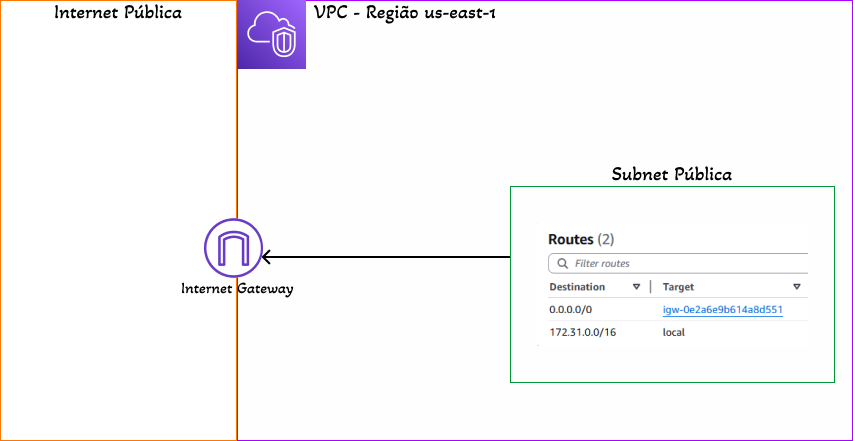
\includegraphics[scale=0.5]{imagens/SubnetPublica.png}
\legend{A rota \texttt{0.0.0.0/0} encaminha o tráfego para o \textit{Internet Gateway} (IGW). 
Ao associar esta tabela à subnet, ela se torna \textbf{pública}.}
\end{figure}


\subsection{Subnet Privada}
Esta subnet hospeda recursos que \textbf{não devem ser expostos diretamente à internet}. Aqui, o tráfego é \textbf{somente de dentro para fora} (saída); conexões \textbf{de fora para dentro} não entram pela internet pública, pois a rota default aponta para um \textit{NAT Gateway}, e não para o \textit{Internet Gateway}.

\Needspace{2\baselineskip}
\begin{lstlisting}[language=YAML,float=htbp,label={lst:subnet-priv-a}]
AppPrivateSubnetA:
  Type: AWS::EC2::Subnet
  Properties:
    AvailabilityZone: !Select [0, !GetAZs '']
    VpcId: !Ref VPC
    CidrBlock: 10.16.32.0/20
    Tags: [{ Key: Name, Value: AppPrivateSubnetA }]
\end{lstlisting}

\begin{description}
  \item[\textbf{AvailabilityZone: !Select [0, !GetAZs '']}] fixa a subnet na \textbf{primeira AZ} da região (índice 0), garantindo distribuição determinística.
  \item[\textbf{VpcId: !Ref VPC}] cria a subnet \textbf{dentro} da VPC definida.
  \item[\textbf{CidrBlock: 10.16.32.0/20}] bloco IP sem sobreposição com as demais sub-redes (recorte do /16 da VPC).
\end{description}

Para saída segura (updates, pull de imagem, etc.), usamos um \textbf{NAT Gateway} com um \textbf{EIP} (IP público fixo). O NAT fica em \textbf{subnet pública} e não aceita conexões iniciadas de fora para dentro, ele apenas \textbf{traduz} o tráfego \emph{originado} das subnets privadas.

\Needspace{2\baselineskip} % reserva espaço; ajuste o 2 se precisar
\begin{lstlisting}[language=YAML, float=htbp]
NatEIPA:
  Type: AWS::EC2::EIP
  Properties:
    Domain: vpc
\end{lstlisting}

\begin{description}
  \item[\textbf{Domain: vpc}] aloca o EIP no escopo da \textbf{VPC}. Esse EIP será o \textbf{IP público fixo} do NAT.
\end{description}

\Needspace{2\baselineskip} % reserva espaço; ajuste o 2 se precisar
\begin{lstlisting}[language=YAML, float=htbp]
NATGWA:
  Type: AWS::EC2::NatGateway
  Properties:
    AllocationId: !GetAtt NatEIPA.AllocationId
    SubnetId: !Ref PublicSubnetA
    Tags: [{ Key: Name, Value: NATGW-A }]
\end{lstlisting}

\begin{description}
  \item[\textbf{AllocationId: !GetAtt NatEIPA.AllocationId}] \textbf{vincula} o EIP ao NAT (garante IP público estável para o tráfego de saída).
  \item[\textbf{SubnetId: !Ref PublicSubnetA}] o NAT \textbf{deve ficar em subnet pública} (pois precisa falar com a internet via IGW).
\end{description}

Criamos então a \textbf{route table privada} da AZ A e apontamos a \textbf{rota default (0.0.0.0/0)} para o \textbf{NAT Gateway}, é isso que dá à subnet privada \textbf{saída para a internet} sem exposição de entrada.

\Needspace{2\baselineskip} % reserva espaço; ajuste o 2 se precisar
\begin{lstlisting}[language=YAML, float=htbp]
PrivateRTA:
  Type: AWS::EC2::RouteTable
  Properties:
    VpcId: !Ref VPC
    Tags: [{ Key: Name, Value: Private-RT-A }]
\end{lstlisting}

\Needspace{2\baselineskip} % reserva espaço; ajuste o 2 se precisar
\begin{lstlisting}[language=YAML, float=htbp]
PrivateDefaultRouteA:
  Type: AWS::EC2::Route
  Properties:
    RouteTableId: !Ref PrivateRTA
    DestinationCidrBlock: 0.0.0.0/0
    NatGatewayId: !Ref NATGWA
\end{lstlisting}

\begin{description}
  \item[\textbf{RouteTableId: !Ref PrivateRTA}] indica \textbf{em qual tabela} a rota será criada (a “privada A”).
  \item[\textbf{DestinationCidrBlock: 0.0.0.0/0}] \textbf{tudo que não for rede interna} (default) segue esta rota.
  \item[\textbf{NatGatewayId: !Ref NATGWA}] define o \textbf{alvo} da default como o NAT (saída \emph{egress} apenas).
\end{description}

Por fim, associamos a \textbf{subnet privada} à \textbf{sua route table privada} (mesma lógica do caso público; só mudamos IGW→NAT). Sem essa associação, a subnet herdaria a \textit{main route table}.

\Needspace{2\baselineskip} % reserva espaço; ajuste o 2 se precisar
\begin{lstlisting}[language=YAML, float=htbp]
AssocAppAtoRTA:
    Type: AWS::EC2::SubnetRouteTableAssociation
    Properties:
      SubnetId: !Ref AppPrivateSubnetA
      RouteTableId: !Ref PrivateRTA
\end{lstlisting}

\subsection{Visão Geral Privada}
A seguir, a Figura~\ref{fig:rt-privada} apresenta a parte \textbf{privada} da arquitetura:
a subnet de aplicação com rota \texttt{0.0.0.0/0} apontando para o \textbf{NAT Gateway}.

\begin{figure}[H]
\centering
\caption{Route table \textbf{privada} com rota \texttt{0.0.0.0/0} para o NAT Gateway}
\label{fig:rt-privada}
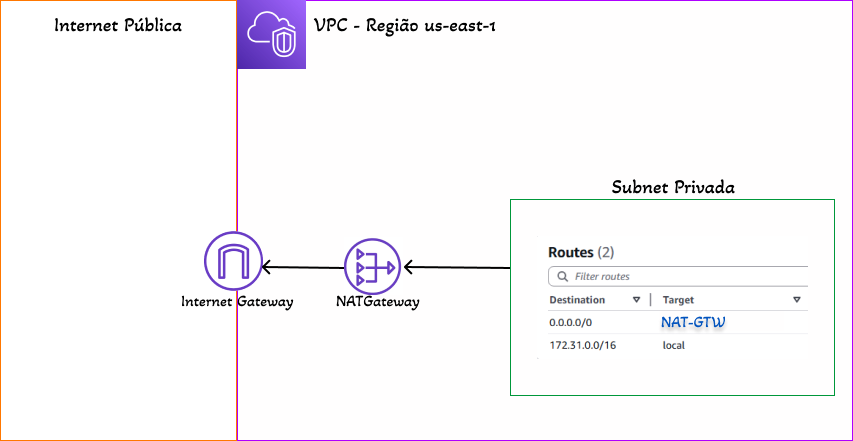
\includegraphics[scale=0.5]{imagens/SubnetPrivada.png}
\legend{A default \texttt{0.0.0.0/0} vai para o \textbf{NAT Gateway} (na subnet pública da \textbf{mesma AZ}),
garantindo \textbf{saída} à Internet via IGW sem expor \textbf{entrada} direta.}
\end{figure}


\section{Grupos de Segurança}
Precisamos criar \textit{Security Groups} (SGs), que são nossos firewalls com estado dentro da VPC. Eles protegem o tráfego e também servem como referência entre recursos: eu defino que “só quem estiver no SG X pode falar com o recurso Y”. Assim, controlo entrada e saída de forma simples e direta, sem abrir portas desnecessárias.

Vamos usar SGs para os nossos principais componentes:

\begin{description}
  \item[\textbf{Balanceador de Carga}] Recebe tráfego público (HTTP/HTTPS) e só encaminha para os containers que estiverem no SG permitido.
  \item[\textbf{Instância do Banco de Dados (RDS)}] Não é pública. Aceita conexões apenas do SG dos containers (porta do banco) e, se necessário, do bastion/jump.
  \item[\textbf{ECS Fargate (Containers)}] Fala com o RDS e com o S3 (via endpoint). Só recebe tráfego do SG do balanceador. Saída liberada apenas para o que precisa.
\end{description}

\Needspace{2\baselineskip} % reserva espaço; ajuste o 2 se precisar
\begin{lstlisting}[language=YAML, float=htbp]
SGALB:
    Type: AWS::EC2::SecurityGroup
    Properties:
      GroupDescription: ALB HTTP
      VpcId: !Ref VPC
      SecurityGroupIngress:
        - { IpProtocol: tcp, FromPort: 80, ToPort: 80, CidrIp: 0.0.0.0/0 }
      SecurityGroupEgress:
        - { IpProtocol: -1, FromPort: 0, ToPort: 0, CidrIp: 0.0.0.0/0 }
\end{lstlisting}

\textbf{GroupDescription: ALB HTTP} Cria uma descrição para o nosso Grupo de Segurança.

\textbf{SecurityGroupIngress: - { IpProtocol: tcp, FromPort: 80, ToPort: 80, CidrIp: 0.0.0.0/0 }} Libera \textbf{todo} tráfego de saída (qualquer protocolo/porta/destino)
        
\textbf{SecurityGroupEgress: - { IpProtocol: -1, FromPort: 0, ToPort: 0, CidrIp: 0.0.0.0/0 }} Libera \textbf{todo} tráfego de saída (qualquer protocolo/porta/destino)

\section{S3 Endpoint Gateway}
Criaremos a nosso S3 Endpoint Gateway, precisamos garantir que ele esteja em duas zonas de disponibilidade, para garantir alta disponibilidade.

\begin{figure}[H]
\centering
\caption{Acesso do container ao S3 via \textbf{Gateway Endpoint} (privado, sem IGW/NAT)}
\label{fig:rt-privada}
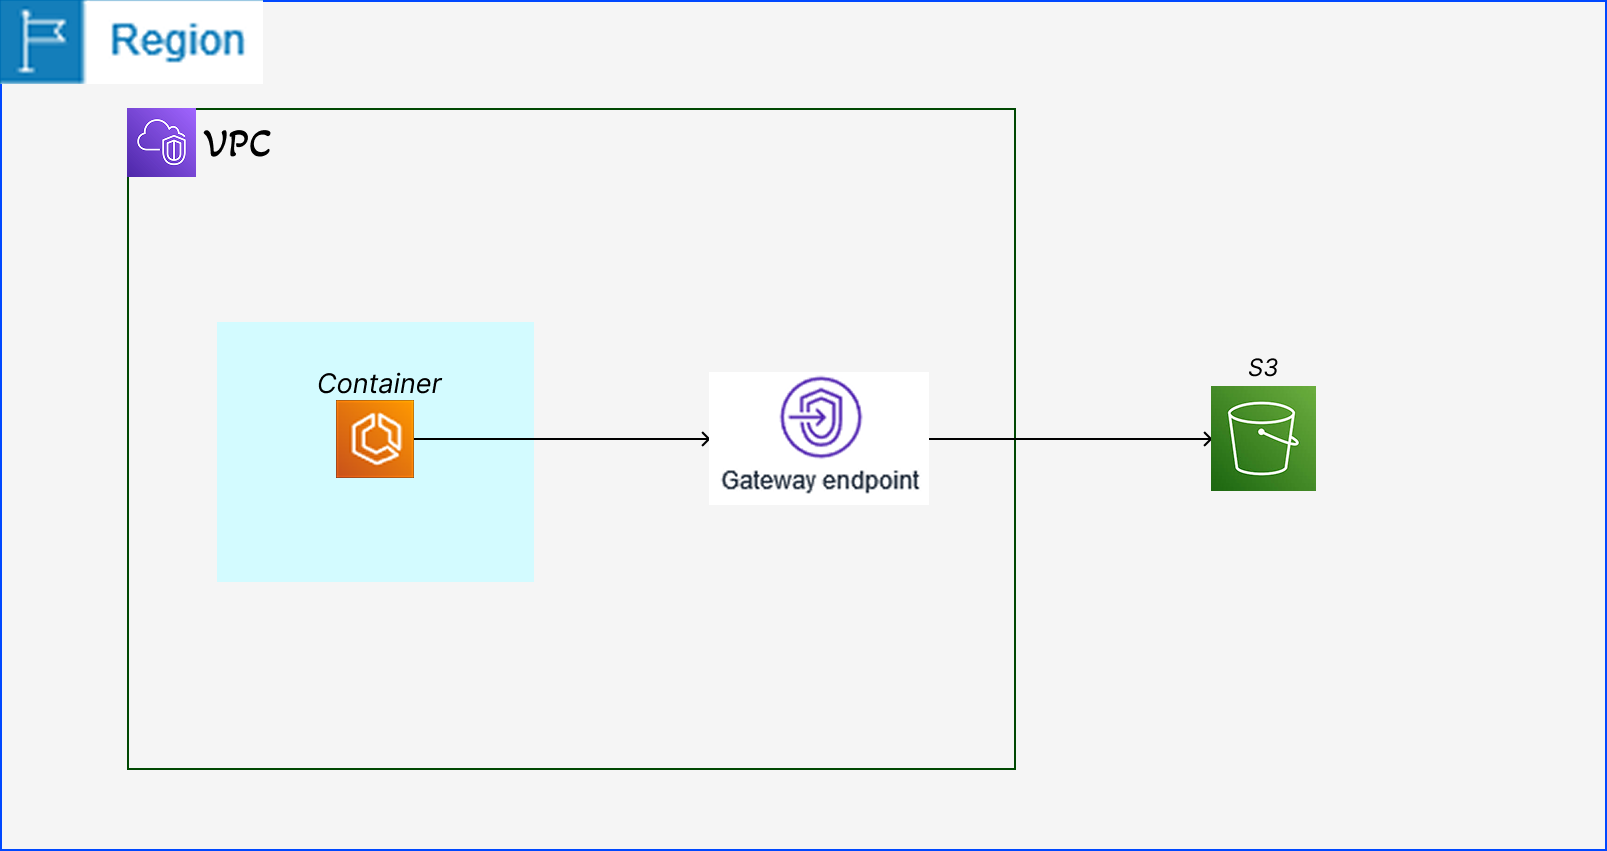
\includegraphics[scale=0.25]{imagens/VPC-Endpoint.png}
\legend{O tráfego ao S3 sai da VPC pelas \textit{route tables} privadas apontando para o \textbf{Gateway Endpoint} do S3. Não há exposição à Internet, nem uso de NAT; o caminho é gerenciado e altamente disponível por padrão.}
\end{figure}

\Needspace{10\baselineskip} % reserva espaço; ajuste o 2 se precisar
\begin{lstlisting}[language=YAML]
S3GatewayEndpoint:
    Type: AWS::EC2::VPCEndpoint
    Properties:
      VpcId: !Ref VPC
      ServiceName: !Sub com.amazonaws.${AWS::Region}.s3
      VpcEndpointType: Gateway
      RouteTableIds: [ !Ref PrivateRTA, !Ref PrivateRTB ]
      PolicyDocument:
        Version: '2012-10-17'
        Statement:
          - Effect: Allow
            Principal: "*"
            Action: "s3:*"
            Resource: "*"
\end{lstlisting}


\textbf{ServiceName: !Sub com.amazonaws.\${AWS::Region}.s3} Nome do serviço do S3 na região (prefix list regional).

\textbf{VpcEndpointType: Gateway} Escolhemos \textit{Gateway} (e não \textit{Interface}) porque é o tipo próprio do S3: usa rotas nas \textit{route tables}, não precisa SG, não exige ENI por AZ e não tem cobrança por hora do endpoint — fica mais simples e barato pro nosso caso.

\textbf{RouteTableIds: [ PrivateRTA, PrivateRTB ]} Associa o endpoint às RTs privadas; assim, o tráfego pro S3 sai por caminho privado (sem IGW/NAT).

\textbf{PolicyDocument} É a política anexada ao recurso, nesse caso o endpoint. Define quem pode usar este caminho privado e para quais ações no S3.

\textbf{Version: \texttt{2012-10-17}} Versão do schema da política da AWS. Mantemos este valor porque é o padrão atual da linguagem de políticas.

\textbf{Statement} Bloco que contém as regras.

\textbf{Effect: \texttt{Allow}} Diz que a regra \textit{permite}. Se fosse \texttt{Deny}, bloquearia, independentemente de outras permissões.

\textbf{Principal: \texttt{"*"}} Quem está autorizado a usar o recurso. Com asterisco, qualquer principal autenticado que alcance o recurso na VPC pode tentar usar.

\textbf{Action: \texttt{"s3:*"}} Conjunto de operações no S3 liberadas por este caminho. Com asterisco, libera todas as ações.

\textbf{Resource: \texttt{"*"}} Alvos das ações. Com asterisco, vale para qualquer bucket e qualquer objeto, tendo a opção de restriginr os recursos, separando por pastas.

\section{Balanceador de Carga}
Aqui é a “porta de entrada” do usuário. O ALB recebe as requisições e distribui entre os nossos containers. Quando utilizamos o cloudformation, é separado em três partes.

\subsection{Load Balancer}
Nesta etapa criamos o recurso principal do balanceador e definimos as características base.\\

\Needspace{10\baselineskip}
\begin{lstlisting}[language=YAML]
ALB:
  Type: AWS::ElasticLoadBalancingV2::LoadBalancer
  Properties:
    Scheme: internet-facing
    Type: application
    Subnets: [ !Ref PublicSubnetA, !Ref PublicSubnetB ]
    SecurityGroups: [ !Ref SGALB ]
\end{lstlisting}

\textbf{Scheme: internet-facing} É o nosso ponto público. Como o usuário acessa de fora, o ALB precisa ser \textit{internet-facing}. Se fosse \textit{internal}, ficaria restrito à VPC.

\textbf{Type: application} Escolhemos \textit{application} (ALB), que trabalha em camada 7 (HTTP/HTTPS) e entende coisas como caminho, host e headers. O outro tipo é \textit{network} (NLB), camada 4, focado em TCP/UDP e baixa latência.

\textbf{Subnets: [ !Ref PublicSubnetA, !Ref PublicSubnetB ]} Colocamos o ALB em subnets \textbf{públicas} de duas AZs para alta disponibilidade e IPs públicos gerenciados.

\textbf{SecurityGroups: [ !Ref SGALB ]} SG anexado ao ALB.

\subsection{Listener}
É o ponto onde o balanceador de carga escuta as requisições. Aqui se define de onde virão e como serão atendidas as requisições dos clientes.\\

\Needspace{10\baselineskip}
\begin{lstlisting}[language=YAML]
Listener80:
  Type: AWS::ElasticLoadBalancingV2::Listener
  Properties:
    LoadBalancerArn: !Ref ALB
    Port: 80
    Protocol: HTTP
    DefaultActions:
      - Type: forward
        TargetGroupArn: !Ref TargetGroup
\end{lstlisting}

\textbf{LoadBalancerArn: !Ref ALB} Referencia em qual balanceador de carga o listener será criado.

\textbf{Port: 80} Informa a porta que será escutada.

\textbf{Protocol: HTTP} Define o protocolo que será escutado.

\textbf{DefaultActions:} Define o que fazer com as requisições que chegarem.

\textbf{- Type: forward} Diz que as requisições devem ser encaminhadas.

\textbf{TargetGroupArn: !Ref TargetGroup} Indica para onde o tráfego será encaminhado.

\subsection{Target Group}
É a forma de agrupar os containers. Ao criar os containers, eles são associados a um Target Group, e o balanceador usa isso para distribuir as requisições.\\

\Needspace{10\baselineskip}
\begin{lstlisting}[language=YAML]
TargetGroup:
  Type: AWS::ElasticLoadBalancingV2::TargetGroup
  Properties:
    VpcId: !Ref VPC
    Protocol: HTTP
    Port: 8080
    TargetType: ip
    HealthCheckPath: /healthcheck
    Matcher: { HttpCode: 200-399 }
\end{lstlisting}

\textbf{VpcId: !Ref VPC} Define em qual VPC o Target Group está.

\textbf{Protocol: HTTP} Informa o protocolo usado entre o ALB e os destinos.

\textbf{Port: 8080} Porta em que os containers responderão.

\textbf{TargetType: ip} Tipo de destino definido como IP.

\textbf{HealthCheckPath: /healthcheck} Caminho usado para o health check, um “ping” básico para verificar se está respondendo.

\textbf{Matcher: \{ HttpCode: 200-399 \}} Intervalo de códigos considerados sucesso no health check.

\begin{figure}[H]
\centering
\caption{ALB encaminhando tráfego para o \textbf{Target Group} (destinos IP na porta 8080)}
\label{fig:load-balancer}
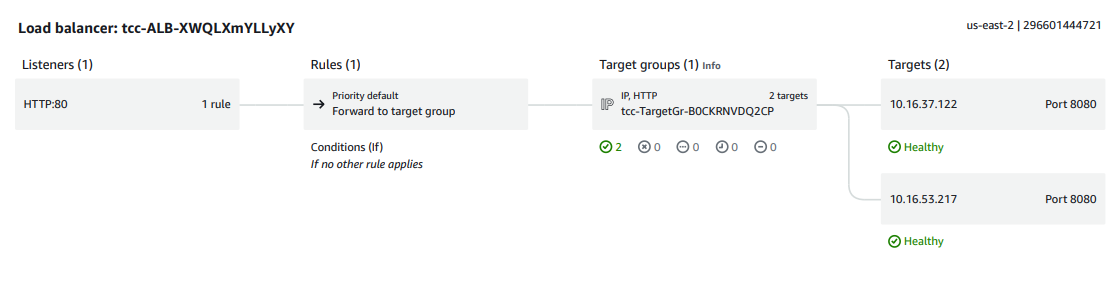
\includegraphics[scale=0.4]{imagens/targets.png}
\legend{Os destinos aparecem como \textit{healthy} após passarem no \textit{health check} definido no Target Group. O balanceamento ocorre a partir do listener HTTP:80.}
\end{figure}

\section{Armazenamento de Objetos}
Será provisionado um bucket S3 para armazenamento de objetos. 
A seção é dividida em duas partes: a criação do recurso e a definição das permissões.\\

\Needspace{10\baselineskip}
\begin{lstlisting}[language=YAML]
MediaBucket:
    Type: AWS::S3::Bucket
    Properties:
      BucketName: !If
        - HasBucketName
        - !Ref MediaBucketName
        - !Sub tcc-flask-media-${AWS::AccountId}-${AWS::Region}
\end{lstlisting}

\textbf{BucketName: !If}

\textbf{ - HasBucketName,} 

\textbf{ - \!Ref MediaBucketName,}

\textbf{ - \!Sub tcc-flask-media-\${AWS::AccountId}-\${AWS::Region}}

Define o nome do bucket. Se um nome for informado no parâmetro \texttt{MediaBucketName}, usa esse valor. Caso contrário, usa o padrão com conta e região.

\Needspace{10\baselineskip}
\begin{lstlisting}[language=YAML]
MediaBucketPolicy:
    Type: AWS::S3::BucketPolicy
    Properties:
      Bucket: !Ref MediaBucket
      PolicyDocument:
        Version: '2012-10-17'
        Statement:
          - Sid: DenyInsecureTransport
            Effect: Deny
            Principal: "*"
            Action: "s3:*"
            Resource:
              - !Sub arn:aws:s3:::${MediaBucket}
              - !Sub arn:aws:s3:::${MediaBucket}/*
            Condition:
              Bool: { aws:SecureTransport: "false" }
\end{lstlisting}


\textbf{Bucket: \texttt{!Ref MediaBucket}} Indica em qual bucket a política será anexada.

\textbf{PolicyDocument} Documento da política em si. É aqui que se define o que é permitido ou negado.

\textbf{Version: \texttt{'2012-10-17'}} Versão do formato da política da AWS. Valor padrão, não altera o comportamento das regras.

\textbf{Statement} Conjunto de regras. 

\textbf{Sid} é só um rótulo legível para identificar a regra.

\textbf{Effect} Define o resultado da regra: \texttt{Allow} para permitir, \texttt{Deny} para negar. Neste caso está como \texttt{Deny}.

\textbf{Principal} Quem está fazendo a chamada. O caractere \texttt{"*"} significa “qualquer principal”.

\textbf{Action} Quais operações a regra cobre. \texttt{"s3:*"} significa “todas as ações do S3”.

- !Sub arn:aws:s3:::\${MediaBucket}

- !Sub arn:aws:s3:::\${MediaBucket}/*

\textbf{Resource} Em quais recursos a regra se aplica. Aqui cobre o bucket raiz.


\section{ECS Fargate - Containers}
A criação das instâncias de containers é organizada em cinco partes: (i) o cluster, que concentra a execução; (ii) o destino dos logs, para facilitar análise em caso de falhas; (iii) as credenciais, separadas em duas funções para manter clareza e granularidade; (iv) a definição da task, onde se especificam propriedades do container e variáveis de ambiente; (v) o service, que define sub-redes de lançamento, quantidade de containers e os vínculos. 

\subsection{Cluster}
No contexto do ECS, o \textit{cluster} é o agrupador lógico onde ficam registrados os serviços e as tasks.

\Needspace{10\baselineskip}
\begin{lstlisting}[language=YAML]
ECSCluster:
  Type: AWS::ECS::Cluster
  Properties:
    ClusterName: flask-ecs-cluster
\end{lstlisting}

\textbf{ClusterName: flask-ecs-cluster} Define o nome lógico do cluster onde os serviços e tasks serão executados.

\subsection{Logs}
Logs registram os eventos de execução do container.
 

\Needspace{10\baselineskip}
\begin{lstlisting}[language=YAML]
LogGroup:
  Type: AWS::Logs::LogGroup
  Properties:
    LogGroupName: /ecs/flask
    RetentionInDays: 7
\end{lstlisting}

\textbf{LogGroupName: /ecs/flask} Nome do grupo de logs para registrar a saída dos containers.

\textbf{RetentionInDays: 7} Define retenção de logs por 7 dias.

\subsection{Credencial de Execução}
Função usada pelo \textit{runtime} do ECS/Fargate durante a execução da task.

\Needspace{10\baselineskip}
\begin{lstlisting}[language=YAML]
ECSExecutionRole:
  Type: AWS::IAM::Role
  Properties:
    AssumeRolePolicyDocument:
      Version: '2012-10-17'
      Statement:
        - Effect: Allow
          Principal: { Service: ecs-tasks.amazonaws.com }
          Action: sts:AssumeRole
    ManagedPolicyArns:
      - arn:aws:iam::aws:policy/service-role/AmazonECSTaskExecutionRolePolicy
\end{lstlisting}

\textbf{AssumeRolePolicyDocument} Autoriza o serviço \texttt{ecs-tasks.amazonaws.com} a assumir a função.

\textbf{Action: sts:AssumeRole} É a linha que afirma que o nosso container pode assumir a nossa Role.

\textbf{ManagedPolicyArns} Anexa a política gerenciada usada na execução das tasks.


\subsection{Credencial da Tarefa}
Função assumida pelo processo dentro do container.

\Needspace{2\baselineskip}
\begin{lstlisting}[language=YAML]
ECSTaskRole:
  Type: AWS::IAM::Role
  Properties:
    AssumeRolePolicyDocument:
      Version: '2012-10-17'
      Statement:
        - Effect: Allow
          Principal: { Service: ecs-tasks.amazonaws.com }
          Action: sts:AssumeRole
    Policies:
      - PolicyName: S3UploadsAccess
        PolicyDocument:
          Version: '2012-10-17'
          Statement:
            - Sid: ListOnBucketPrefix
              Effect: Allow
              Action: ["s3:ListBucket"]
              Resource: !Sub arn:aws:s3:::${MediaBucket}
              Condition:
                StringLike:
                  s3:prefix: [ !Sub "${MediaPrefix}/*" ]
            - Sid: RWOnPrefix
              Effect: Allow
              Action: ["s3:GetObject","s3:PutObject","s3:DeleteObject"]
              Resource: !Sub arn:aws:s3:::${MediaBucket}/${MediaPrefix}/*
\end{lstlisting}

\textbf{AssumeRolePolicyDocument} Permite que as tasks assumam a função.

\textbf{Policies \(\rightarrow\) S3UploadsAccess} Concede acesso mínimo necessário ao bucket de mídias. Priorizando segurança.

\textbf{ListOnBucketPrefix} Autoriza listar o bucket apenas no prefixo informado.

\textbf{RWOnPrefix} Autoriza leitura e escrita de objetos somente no prefixo definido.



\subsection{Task}
Descreve como o container será executado: compatibilidade, recursos, rede, permissões.

\begin{lstlisting}[language=YAML]
TaskDefinition:
    Type: AWS::ECS::TaskDefinition
    DependsOn: [ MySQLInstance ]
    Properties:
      RequiresCompatibilities: [ FARGATE ]
      Cpu: 512
      Memory: 1024
      NetworkMode: awsvpc
      ExecutionRoleArn: !GetAtt ECSExecutionRole.Arn
      TaskRoleArn: !GetAtt ECSTaskRole.Arn
      ContainerDefinitions:
        - Name: flask
          Image: !Ref ECRImage
          PortMappings:
            - ContainerPort: 8080
          Environment:
            ...
          LogConfiguration:
            LogDriver: awslogs
            Options:
              awslogs-group: /ecs/flask
              awslogs-region: !Ref AWS::Region
              awslogs-stream-prefix: app
          HealthCheck:
            Command: ["CMD-SHELL", "curl -fsS http://localhost:8080/healthcheck || exit 1"]
            Interval: 30
            Timeout: 5
            Retries: 3
            StartPeriod: 10
\end{lstlisting}

\textbf{DependsOn: [ MySQLInstance]} Garante a ordem de criação: a task só é criada após a instância do banco. 
\textit{Nota:} isso não garante que o banco já esteja “pronto” para conexões; apenas a criação ocorre depois.

\textbf{RequiresCompatibilities: [ FARGATE ]} Define que a execução é no Fargate (sem gerenciamento de servidor).

\textbf{Cpu: 512} Quantidade de CPU reservada para a task.

\textbf{Memory: 1024} Quantidade de memória reservada para a task (em MiB).

\textbf{NetworkMode: awsvpc} Modo de rede compatível com Fargate. Cada task tem endereço IP próprio na VPC e pode usar Security Group dedicado.

\textbf{ExecutionRoleArn: !GetAtt ECSExecutionRole.Arn} Função usada pelo runtime do ECS (pull da imagem, logs, etc.).

\textbf{TaskRoleArn: !GetAtt ECSTaskRole.Arn} Função assumida pelo processo dentro do container (permissões da aplicação; no caso, acesso ao S3).

\textbf{ContainerDefinitions} Bloco com as características do container que vai rodar.

\quad\textbf{Name: flask} Nome lógico do container.

\quad\textbf{Image: !Ref ECRImage} Imagem utilizada no deploy.

\quad\textbf{PortMappings \(\rightarrow\) ContainerPort: 8080} Porta na qual o container escuta.

\quad\textbf{Environment} Bloco de variáveis de ambiente do container.

\quad\textbf{LogConfiguration \(\rightarrow\) LogDriver: awslogs} Envio de logs para o CloudWatch Logs (\texttt{group}, \texttt{region}, \texttt{stream-prefix}).

\quad\textbf{HealthCheck} Comando para verificação de saúde do container (intervalo, timeout, tentativas e período inicial)..

\subsection{Service}
Definimos a quantidade de instâncias que vamos lançar, as subnets e outros.

\begin{lstlisting}[language=YAML]
Service:
    Type: AWS::ECS::Service
    DependsOn: [ ALB, Listener80, TargetGroup ]
    Properties:
      Cluster: !Ref ECSCluster
      LaunchType: FARGATE
      DesiredCount: 2
      EnableExecuteCommand: true
      TaskDefinition: !Ref TaskDefinition
      NetworkConfiguration:
        AwsvpcConfiguration:
          AssignPublicIp: DISABLED
          Subnets: [ !Ref AppPrivateSubnetA, !Ref AppPrivateSubnetB ]
          SecurityGroups: [ !Ref APPSG ]
      LoadBalancers:
        - ContainerName: flask
          ContainerPort: 8080
          TargetGroupArn: !Ref TargetGroup
\end{lstlisting}

\textbf{DependsOn: [ ALB, Listener80, TargetGroup ]} Garante a criação do ALB, listener e target group antes do service.

\textbf{Cluster: !Ref ECSCluster} Agrupamento onde o service será executado.

\textbf{LaunchType: FARGATE} Tipo de execução do container.

\textbf{DesiredCount: 2} Quantidade de instâncias (tasks) em execução.

\textbf{EnableExecuteCommand: true} Habilita comandos interativos na task (exec).

\textbf{TaskDefinition: !Ref TaskDefinition} Qual definição de task o service vai usar.

\textbf{NetworkConfiguration \(\rightarrow\) AwsvpcConfiguration}
\quad \textbf{AssignPublicIp: DISABLED} Sem IP público para as tasks.

\quad \textbf{Subnets: [ AppPrivateSubnetA, AppPrivateSubnetB ]} Sub-redes privadas onde as tasks serão lançadas.

\quad \textbf{SecurityGroups: [ APPSG ]} Grupo de segurança aplicado nas tasks.

\textbf{LoadBalancers}
\quad \textbf{ContainerName: flask} Container dentro da task que receberá o tráfego.

\quad \textbf{ContainerPort: 8080} Porta do container exposta ao ALB.

\quad \textbf{TargetGroupArn: !Ref TargetGroup} Para onde o ALB encaminha as requisições.


\section{Banco de Dados}
A criação do banco é dividida em duas etapas: primeiro o \textit{Subnet Group}, que define onde a instância pode ser alocada; depois a própria instância, com suas propriedades.

\subsection{Subnet Group — Banco de Dados}

\Needspace{3\baselineskip}
\begin{lstlisting}[language=YAML]
DBSubnetGroup:
  Type: AWS::RDS::DBSubnetGroup
  Properties:
    DBSubnetGroupDescription: Subnets para RDS MySQL
    SubnetIds: [ !Ref DBPrivateSubnetA, !Ref DBPrivateSubnetB ]
\end{lstlisting}

\textbf{DBSubnetGroupDescription: Subnets para RDS MySQL} Descrição do grupo de sub-redes.\\
\textbf{SubnetIds: [ !Ref DBPrivateSubnetA, !Ref DBPrivateSubnetB ]} Sub-redes onde a instância de banco pode ser criada (duas AZs).

\subsection{Instância - Banco de Dados}
Nesta etapa são definidas as propriedades da instância: versão do SGBD, classe de instância, tamanho e tipo de armazenamento, além dos parâmetros básicos de operação. O objetivo é especificar o que será executado e como será alocado o recurso para atender à aplicação.\\

\Needspace{10\baselineskip}
\begin{lstlisting}[language=YAML]
MySQLInstance:
    Type: AWS::RDS::DBInstance
    Properties:
      Engine: mysql
      EngineVersion: "8.0.42"
      DBInstanceClass: db.t4g.micro
      AllocatedStorage: 20
      StorageType: gp3
      MultiAZ: true
      MasterUsername: !Ref DBUser
      MasterUserPassword: !Ref DBPassword
      DBName: !Ref DBName
      VPCSecurityGroups: [ !Ref DBSG ]
      DBSubnetGroupName: !Ref DBSubnetGroup
\end{lstlisting}

\textbf{Engine: mysql} Motor do banco definido como MySQL.

\textbf{EngineVersion: "8.0.42"} Versão utilizada do MySQL.

\textbf{DBInstanceClass: db.t4g.micro} Classe/tamanho da instância (perfil de demonstração).

\textbf{AllocatedStorage: 20} Armazenamento alocado em GiB.

\textbf{StorageType: gp3} Tipo de volume usado pelo RDS.

\textbf{MultiAZ: true} Habilita implantação em múltiplas zonas de disponibilidade, com failover automático.

\textbf{MasterUsername: !Ref DBUser} Usuário principal do banco.

\textbf{MasterUserPassword: !Ref DBPassword} Senha do usuário principal.

\textbf{DBName: !Ref DBName} Nome do database inicial.

\textbf{VPCSecurityGroups: [ !Ref DBSG ]} Grupo(s) de segurança associados à instância.

\textbf{DBSubnetGroupName: !Ref DBSubnetGroup} Sub-redes onde a instância pode ser criada.

\textbf{CopyTagsToSnapshot: true} Replica as tags da instância para os snapshots.


\section{Parâmetros}
Declara os valores que podem ser informados na criação (ou atualização) da pilha, permitindo personalizar o template conforme a necessidade. São valores fornecidos em tempo de implantação e depois referenciados no template pelos recursos que precisam deles.
 
\Needspace{10\baselineskip}
\begin{lstlisting}[language=YAML]
Parameters:
  ECRImage:
    Type: String
    Default: 296601444721.dkr.ecr.us-east-2.amazonaws.com/tcc/flask:latest

  DBName:
    Type: String
    Default: appdb
    Description: Nome do database no RDS MySQL

  DBUser:
    Type: String
    Default: appuser
    Description: Usuário do DB

  DBPassword:
    Type: String
    NoEcho: true
    Description: Senha do DB (8-41 chars)

  MediaBucketName:
    Type: String
    Default: ""
    Description: Nome do bucket S3 para mídias; Em branco, cria um aleatório 

  MediaPrefix:
    Type: String
    Default: "uploads"
    Description: Prefixo (caminho) para objetos no S3

Conditions:
  HasBucketName: !Not [ !Equals [ !Ref MediaBucketName, "" ] ]
\end{lstlisting}


\textbf{ECRImage} Nome do parâmetro usado para referência no template (via \texttt{!Ref}); aqui guarda a URI da imagem no ECR.

\textbf{Type: String} Tipo do parâmetro no CloudFormation. Existindo. Há String e Number.

\textbf{Default: 296601444721.dkr.ecr.us-east-2.amazonaws.com/tcc/flask:latest} Valor padrão. Se o usuário não informar nada, será usada essa imagem Docker.